\chapter{Kako poredimo biološke sekvence?}
\setbookcodestyle

\section{Biološki uvid u poređenje sekvenci}

Kako su biološke sekvence podložne promeni, umetanju i brisanju, čest je slučaj da i-ti simbol jedne sekvence odgovara simbolu na drugoj poziciji druge sekvence. U tom slučaju, cilj je postići najbolje poklapanje simbola.
Na primer, $ATGCATGC$ i $TGCATGCA$ nemaju delove koji se poklapaju, pa je njihova Hamingova udaljenost 8:

\begin{center}
$ATGCATGC$\\
$TGCATGCA$
\end{center}
    
Ali ako ih malo drugačije poravnamo, ove dve niske imaju 6 poklapajucih pozicija:

\begin{center}
$A\textcolor{red}{TGCATGC}-$\\
$-\textcolor{red}{TGCATGC}A$
\end{center}

Stringovi ATGCTTA i TGCATTAA imaju manje uocljive slicnosti:

\begin{center}
$A\textcolor{red}{TGC}-\textcolor{red}{TTA}-$\\
$-\textcolor{red}{TGC}A\textcolor{red}{TTA}A$
\end{center}

Ovi primeri navode nas da definisemo dobro poravnanje kao ono koje ima najveći mogući broj poklapanja. Povećanje broja poklapanja simbola možemo posmatrati kao igricu u kojoj u svakom potezu imamo dva izbora. Možemo da uklonimo oba simbola i osvojimo poen ako su oni isti ili mozemo ukloniti simbol iz jedne od niski, ne osvojimo poene, ali omogućimo da u daljem igranju osvojimo više poena. Cilj je da maksimizujemo broj poena.


%%%%%%%%%%%%%%%%%%%%%%%% ALEX
\section{Igra poravnanja i najduža zajednička podsekvenca}

Kod \textbf{Igre poravnanja} cilj je ukloniti sve simbole iz
sekvenci tako da pritom sakupimo što više poena :
\begin{itemize}
    \item Uklanjanje prvog simbola iz svake sekvence
            \item \textcolor{red}{1} poen ako se simboli poklapaju,  \textcolor{purple}{0} ako se simboli ne poklapaju
    \item Uklanjanje prvog simbola iz jedne sekvnce
         \begin{itemize}
            \item 0 poena
        \end{itemize}
\end{itemize}

\begin{figure}[h!]
\centering
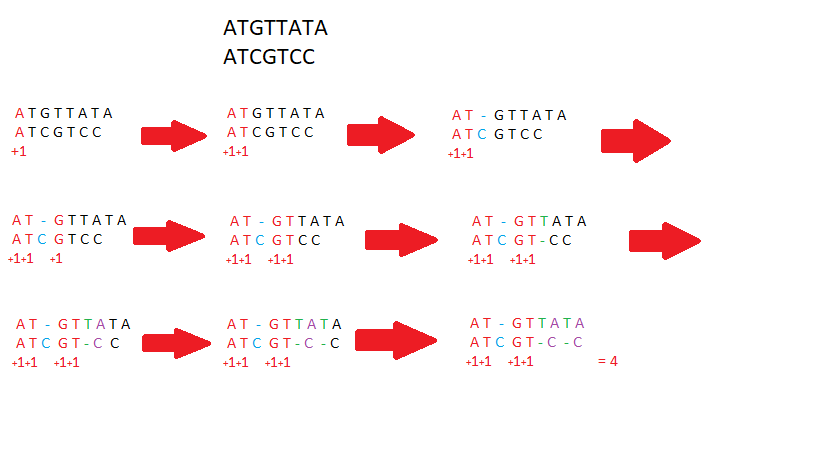
\includegraphics[width=0.7\textwidth]{poglavlja/5/slike/igraPoravnavanja.png}
\caption{Igra poravnanja}
\end{figure} 

\textbf{Poravnanje} dve sekvence predstavlja matricu koja ima dva reda:

\begin{enumerate}
    \item red: simboli prve sekvence (redom) eventualno sa ubačenim “-” 
    \item red: simboli druge sekvence (redom) eventualno sa ubačenim “-” 
\end{enumerate}
\begin{figure}[h!]
\centering
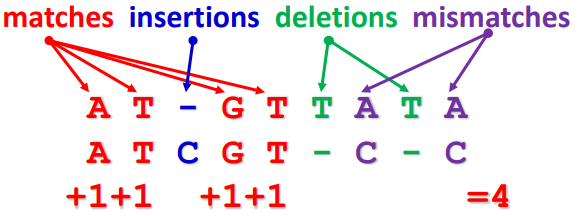
\includegraphics[width=0.4\textwidth]{poglavlja/5/slike/poravnanje.png}
\caption{Poravnanje}
\label{slika:poravnavanje}
\end{figure} 

\subsection{Najduža zajednička podsekvenca}

Poklapanja (matches) u poravnanju dve sekvence ( u primeru \ref{slika:poravnavanje} to je ATGT) formiraju njihovu zajedničku podsekvencu.
\begin{problem}[Problem najduže zajedničke podniske]
	Naći najdužu zajedničku podsekvencu dve niske. \\
	Ulaz: Dve niske. \\
	Izlaz: Najduža zajednička podsekvenca ovih niski
\end{problem}
%%%%%%%%%%%%%%%%%%%%%%%%%%%%%%%%%%%%%%%%%%%%

\section{Problem turiste na Menhetnu}

\noindent Pre svega postavimo problem:\\

\begin{problem}[Problem turiste na Menhetnu]
	Naći najdužu putanju u pravougaonoj mreži gradskih ulica. \\
	Ulaz: Usmeren težinski mrežni graf. \\
	Izlaz: Najduža putanja od početnog (source) do krajnjeg čvora (sink) u mrežnom grafu. 
\end{problem}

\begin{figure}[h!]
\centering
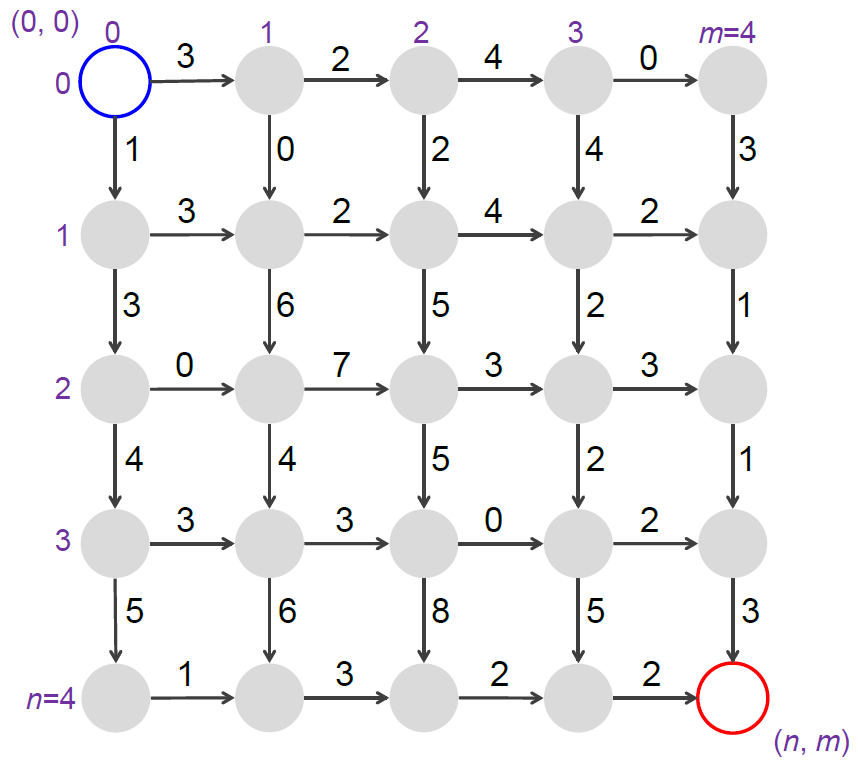
\includegraphics[width=0.7\textwidth]{poglavlja/5/slike/menhetn2.png}
\caption{Problem turiste na Menhetnu}
\label{slika:menhetn}
\end{figure} 

Na slici \ref{slika:menhetn} grafički je prikazan problem turiste na Menhetnu. Cilj je stići od plavog do crvenog kruga i pri tom sakupiti što više poena. Dozvoljeno kretanje je dole i desno. Možemo koristiti pohlepni algoritam i tako doći do cilja, ali da li smo tako sakupili najviše poena?

\noindent Dodatna izmena grafa bi bila da imamo i dijagnalne grane (\ref{slika:menhetn3}).

\begin{figure}[h!]
\centering
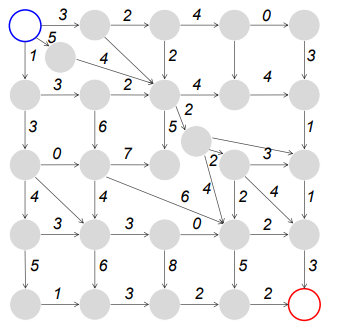
\includegraphics[width=0.7\textwidth]{poglavlja/5/slike/menhetn3.png}
\caption{Nepravilna mreža}
\label{slika:menhetn3}
\end{figure}

\noindent Time dolazimo do sledećeg problema:

\begin{problem}[Problem najduže putanje u usmerenom grafu]
	Naći najdužu putanju između dva   čvora u težinskom usmerenom grafu. \\
	Ulaz: Usmereni težinski graf sa označenim
čvorovima source i sink. \\
	Izlaz: Najduža putanja od čvora source do čvora
sink u usmerenom težinskom grafu. 
\end{problem}

Ako se prisetimo igre poravnanja, videćemo da postoji veza između ova dva problema (igre).

\begin{figure}[h!]
\centering
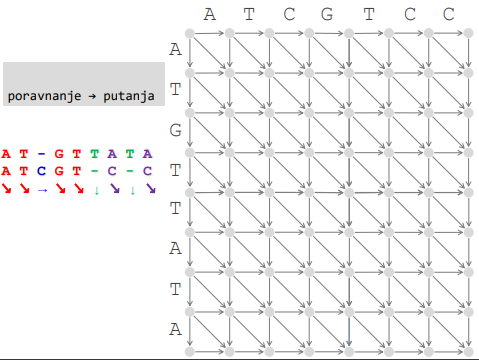
\includegraphics[width=0.7\textwidth]{poglavlja/5/slike/menhetn4.png}
\caption{Poravnanje $\rightarrow$ Putanja}
\label{slika:menhetn4}
\end{figure}

Pitamo se kako izgraditi graf za igru poravnanja i za problem najduže podsekvence. To ćemo uraditi na sledeći način:

\begin{itemize}
    \item Vrste označimo aminokiselinama iz prve niske
    \item Kolone označimo aminokiselinama iz druge niske
    \item U svaku presečnu tačku postavimo jedan čvor
    \item Gde god je moguće, postaviti vertikalne (insercija), horizontalne (delecija) i dijagonalne grane (match ili mismatch)
    \item Dijagonalne grane otežati koeficijentom 1, ostale koeficijentom 0
    \item Problem najduže zajedničke podsekvence se svodi na problem nalaženja najduže putanje između dva data čvora u usmerenom grafu
\end{itemize}

Kada nađemo poravnanje najvišeg skora našli smo i najdužu putanju u mrežnom grafu.

\begin{figure}[h!]
\centering
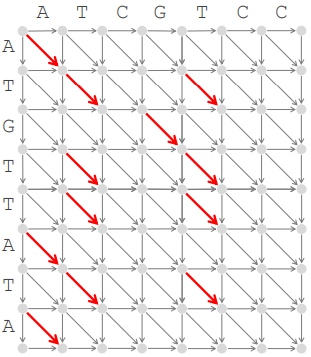
\includegraphics[width=0.7\textwidth]{poglavlja/5/slike/poravnanje1.png}
\caption{Poravnanje $\rightarrow$ Putanja}
\label{slika:poravnanje2}
\end{figure}

Dijagonalne crvene grane odgovaraju poklapanju simbola i imaju skor 1 (\ref{slika:poravnanje2})

%%%%%%%%%%%%%%%%%%%%%%%%%%%%%%%%%%%%%jasmina%%%%%%%%%%%%%%%%%%%%%%%%%%%%%%%%%%%%%%%%%%%%%%%%%%%%%%%%%%%%%%%%%%%%%%%%%%%%%%%%%%%%%%%%%%%%%%%%%%%%%%%%
\section{Problem kusura}

\noindent Upoznajmo se sa sledećim problemom:\\

\begin{problem}[Problem vraćanja kusura]
	Naći minimalan broj novčića neophodnih za vraćanje kusura. \\
	Ulaz: Ceo broj money i niz pozitivnih celih brojeva $(coin_1, coin_2, ..., coin_d)$. \\
	Izlaz: Minimalan broj novčića $(coin_1, coin_2, ..., coin_d)$ u apoenima koji rasitnjava sumu money. \\
\end{problem}

\subsection{Pohlepni algoritam}

Najzastupljeniji način vraćanja kusura širom sveta podrazumeva iterativno traženje sledećeg najvećeg novčića.\\
To bi značilo da bismo za kusur od 42 dinara dobili sledeće novčiće: 20 + 10 + 10 + 2. \\
Ovakav način vraćanja kusura opisuje takozvani pohlepni algoritam. \\

\begin{lstlisting}
GreedyChange(money)
begin
    change %$\leftarrow$% empty collection of coins
	while money > 0
		coin %$\leftarrow$% largest denomination that does not exceed money
		add coin to change
		money %$\leftarrow$% money - coin
	return change
end
\end{lstlisting}

Međutim, ako malo bolje razmislimo ovo rešenje zapravo nije najbolje.\\
Kusur bismo mogli vratiti i sa manje novčića na sledeći način: 42 = 20 + 20 + 2 \\

\textit{Zaključak}: \textbf{GreedyChange ne daje optimalno rešenje!}

\subsection{Rekurzivni algoritam}

Pokušajmo sada da problem rešimo na drugačiji način koristeći rekurziju. \\
Za zadate apoene 6, 5, 1, koji je najmanji broj novčića neophodnih za vraćanje kusura od 9 centi? \\

\begin{figure}[h!]
\centering
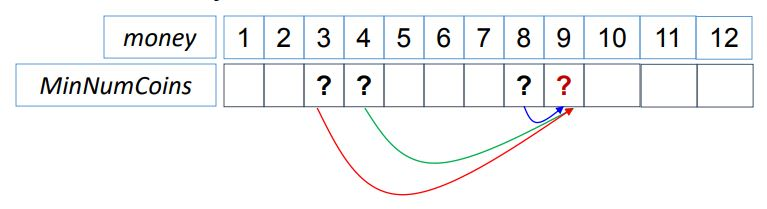
\includegraphics[width=0.7\textwidth]{poglavlja/5/slike/rekurzija1.JPG}
\caption{Vracanje kusura - rekurzija}
\label{slika:rekurzija}
\end{figure}

Problem resavamo tako sto prvo od 9 oduzmemo 6 i dobijemo 3 kao ostatak kusura. Dakle, 9 se može vratiti od jednog novčića od 6 apoena i jos plus broj novčiča koji je potreban za preostali deo kusura od 3 centa. \\
U istoj iteraciji analogno računamo za preostale apoene.\\

Na slici \ref{slika:rekurzija} crvenim znakom pitanja označeno je traženo rešenje koje dobijemo rešavanjem manjih problema za kusure 3, 4 i 8. \\ 

MinNumCoins(9) = $\min$ 
$\begin{cases}$
$MinNumCoins(9-6) + 1 = MinNumCoins(3) + 1\\$
$MinNumCoins(9-5) + 1 = MinNumCoins(4) + 1\\$
$MinNumCoins(9-1) + 1 = MinNumCoins(8) + 1\\$
$\end{cases}$

Na osnovu prethodnog, moguće je izvesti opštu formulu:

MinNumCoins(money) = $\min$ 
$\begin{cases}$
$MinNumCoins(money-coin_{1}) + 1 \\$
$\dots \\$
$MinNumCoins(money-coin_{d}) + 1 \\$
$\end{cases}$
\\
Hajde sada da vidimo kako bismo to isprogramirali:
\\
\begin{lstlisting}
RecursiveChange(money, coins)
begin
    if money = 0
        return 0
    MinNumCoins %$\leftarrow$% infinity 
    for i %$\leftarrow$% 1 to |coins|
        if money %$\geq coin_{i}$%
            NumCoins %$\leftarrow$% RecursiveChange(money - %$coin_{i}$%, coins)
            if numCoins + 1 < MinNumCoins
                MinNumCoins %$\leftarrow$% numCoins + 1
	return MinNumCoins
end
\end{lstlisting}

Reklo bi se da smo sada dobili odgovarajuci algoritam za naš problem, hajde to da proverimo. \\
Postavlja se pitanje, koliko je brz RecursiveChange? \\

Pokušajmo na konkretnom primeru da dođemo do rešenja. Neka naš problem sada bude vraćanje kusura od 76 centi. Pomoću rekurzivnog stabla demonstrirajmo ponašanje našeg algoritma: \\

\begin{figure}[h!]
\centering
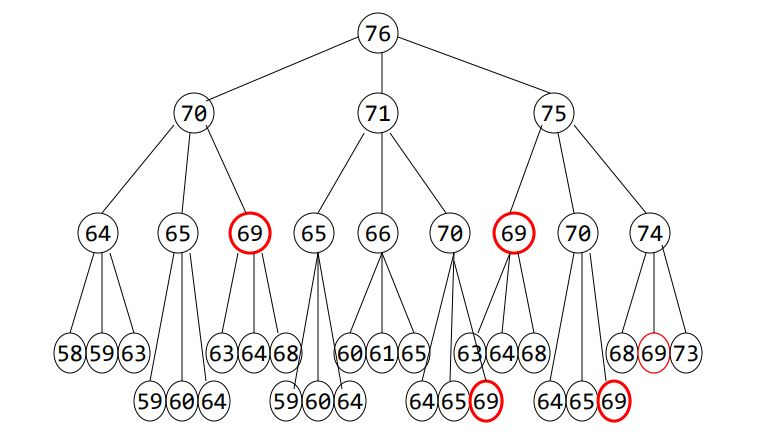
\includegraphics[width=0.7\textwidth]{poglavlja/5/slike/rekurzivnoStablo.JPG}
\caption{Vracanje kusura - ponašanje rekurzivnog algoritma}
\label{slika:rekurzija2}
\end{figure}

Ono što se odmah može primetiti jeste višestruko pozivanje algoritma za vrednost od 69 centi, čak 6 puta! \\
Daljim procenama možemo doći do zaključka da se optimalna kombinacija novčića za 30 centi izračunava milijardama puta! \\

Sada je očigledno da nam rekurzija ne rešava problem na najbolji mogući način. \\

\subsection{Vraćanje kusura dinamičkim programiranjem}

Cilj nam je da izbegnemo višestruka izračunavanja  vraćanja kusura za istu vrednost, tako da bi ideja bila da imamo objekat koji će pamtiti sva računanja i iz koga ćemo čitati već izračunate vrednosti. \\
Dakle, umesto vremenski zahtevnih poziva \\
\begin{center}
RecursiveChange(money - $coin_{i}$, coins)
\end{center}
jednostavno bismo potražili vrednosti iz unapred izračunate tabele \\
\begin{center}
MinNumCoins(money - $coin_{i}$).
\end{center}


\begin{lstlisting}
DPChange(money, coins)
begin
    MinNumCoins(0) %$\leftarrow$% 0 
    for m %$\leftarrow$% 1 to money
        MinNumCoins(m) %$\leftarrow$% infinity
        for i %$\leftarrow$% 1 to |coins|
            if m %$\geq coin_{i}$%
                if MinNumCoins(m - %$coin_{i}$%) + 1 < MinNumCoins(m)
                    MinNumCoins(m) %$\leftarrow$% MinNumCoins(m - %$coin_{i}$%) + 1
	return MinNumCoins(money)
end
\end{lstlisting}


\section{Dinamičko programiranje i putokazi za povratak}

Posmatramo jednostavniji, Menhetn graf:
Pretpostavimo da do čvora sink možemo doći samo na dva načina: kretanjem južno $\downarrow$ ili kretanjem istočno $\rightarrow$

\begin{figure}[h!]
\centering
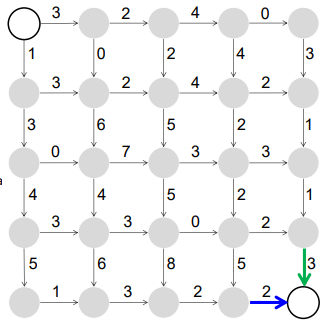
\includegraphics[width=0.7\textwidth]{poglavlja/5/slike/putokazi.png}
\caption{Južno ili istočno?}
\label{slika:putokazi}
\end{figure}

\noindent Prvo probamo da rešimo problem rekurzivno:

\begin{lstlisting}
SouthOrEast(n, m)
if n=0 and m=0
    return 0
x %$\leftarrow$% -infinity, y %$\leftarrow$% -infinity
if n > 0
x %$\leftarrow$% SouthOrEast(n-1,m)+weight of edge "%$\downarrow$%" into (n, m)
if m > 0
y %$\leftarrow$% SouthOrEast(n,m-1)+ weight of edge "%$\rightarrow$%" into (n,m)
return max{x, y}
\end{lstlisting}

\noindent Ovaj algoritam se poziva za svaki čvor u grafu veličine $m\times n$, a pri tom se dešava da za jedan isti čvor računamo više puta. Zbog toga je ovaj pristup previše spor, pa prelazimo na dinamičko programiranje.
Krenućemo  od početnog čvora. Zatim, u čvor (i, j) upisujemo dužinu maksimalne putanje od (0,0) do (i,j). Prvo izračunamo za čvorove na obodu grafa a zatim, kolonu po kolonu, za preostale čvorove.

\begin{figure}[h!]
\centering
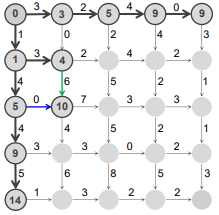
\includegraphics[width=0.5\textwidth]{poglavlja/5/slike/putokazi1.png}
\caption{Južno ili istočno?}
\label{slika:putokazi1}
\end{figure}

\begin{figure}[h!]
\centering
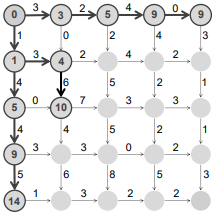
\includegraphics[width=0.5\textwidth]{poglavlja/5/slike/putokazi2.png}
\caption{Južno ili istočno?}
\label{slika:putokazi2}
\end{figure}

\begin{figure}[h!]
\centering
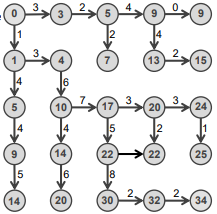
\includegraphics[width=0.5\textwidth]{poglavlja/5/slike/putokazi3.png}
\caption{Južno ili istočno?}
\label{slika:putokazi3}
\end{figure}

Na slici \ref{slika:putokazi3} prikazane su podebljane grane koje predstavljaju putokaze za povratak od čvora sink do čvora source.

\subsection{Rekurentna relacija dinamičkog programiranja kod Menhetn grafa}

$s_i,_j$: the length of a longest path from (0,0) to (i,j)

$s_i,_j$ = $\max$ $\begin{cases}$
$s_{i-1},_j + weight of edge "\downarrow"into (i,j)\\$
$s_i,_{j-1} + weight of edge "\rightarrow"into (i,j)$
$\end{cases}$

\begin{lstlisting}
ManhattanTourist(n, m, Down, Right)
%$s_0,_0$% %$\leftarrow$% 0
for i %$\leftarrow$% 1 to n
    %$s_i,_0$% %$\leftarrow$% %$s_{i-1},_0$% + %$down_i,_0$%
for j %$\leftarrow$% 1 to m
    %$s_0,_j$% %$\leftarrow$% %$s_0,_{j-1}$% + %$right_0,_j$% 
for i %$\leftarrow$% 1 to n
    for j %$\leftarrow$% 1 to m
        %$s_i,_j$% %$\leftarrow$% %$\max$% { %$s_{i-1},_j$% + %$down_i,_j$%, %$s_i,_{j-1}$% + %$right_i,_j$% }
return %$s_n,_m$%
\end{lstlisting}



%%%%%%%%%%%%%%%%%%%%%%%%%%%%%%%%%%%%%%%%%%%%%%%%%%%%%%%%%%%%%%%%%%%%%%%%%

\section{Od Menhetna do grafa poravnanja }

\subsection{Rekurentna relacija dinamičkog programiranja kod grafa poravnanja}


Najduži put (slika \ref{slika:povratak}) od (0,0) do (i,j) se računa:


$s_i,_j$ = $\max$ $\begin{cases}$
$s_{i-1},_j$ + 
$\textcolor{green}{weight\ of\ edge\ "\downarrow"\ into\ (i,j)}\\$
$s_i,_{j-1}$ + 
$\textcolor{blue}{weight\ of\ edge\ "\rightarrow"\ into\ (i,j)}\\$
$s_{i-1},_{j-1}$ + 
$\textcolor{red}{weight\ of\ edge\ "\searrow"\ into\ (i,j)}$
$\end{cases}$

Što dalje daje :

$s_i,_j$ = $\max$ $\begin{cases}$
$\textcolor{green}{s_{i-1},_j + 0}\\$
$\textcolor{blue}{s_i,_{j-1} + 0}\\$
$\textcolor{red}{s_{i-1},_{j-1} + 1, v_i = w_j}\\$
$\textcolor{red}{s_{i-1},_{j-1} + 0, v_i \neq w_j}$
$\end{cases}$



\begin{figure}[h!]
\centering
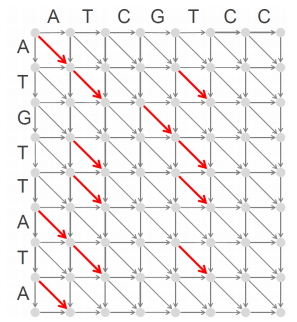
\includegraphics[width=0.5\textwidth]{poglavlja/5/slike/graf1.png}
\caption{ Crvene grane težina 1, ostale grane težina 0, $v_i$ i $w_j$ oznake vrste i kolone}
\label{slika:povratak}
\end{figure}


U slici \ref{slika:backtrack} se vide boldovane grane koje su nastale primenom pravila rekurentne relacije. One predstavljaju putokaze za povratak (backtrack) kod grafa za najdužu zajedničku podsekvencu. 

\begin{figure}[h!]
\centering
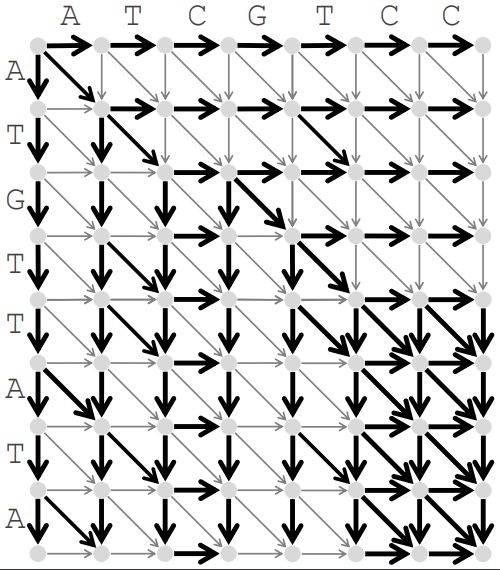
\includegraphics[width=0.5\textwidth]{poglavlja/5/slike/backtrack.png}
\caption{Putokazi za povratak (backtrack)}
\label{slika:backtrack}
\end{figure}

\subsection{Računanje putokaza za povratak }

$s_i,_j$ $\leftarrow$ $\max$ $\begin{cases}$
$\textcolor{green}{s_{i-1},_j + 0}\\$
$\textcolor{blue}{s_i,_{j-1} + 0}\\$
$\textcolor{red}{s_{i-1},_{j-1} + 1, v_i = w_j}\\$
$\textcolor{red}{s_{i-1},_{j-1} + 0, v_i \neq w_j}$
$\end{cases}$


$backtrack_i,_j$  $\leftarrow$  $\max$ $\begin{cases}$
$\textcolor{blue}{ "\rightarrow", s_i,_j = s_{i},_{j-1}}\\$
$\textcolor{green}{ "\downarrow", s_i,_j = s_{i-1},_j}\\$
$\textcolor{red}{"\searrow", otherwise}$
$\end{cases}$


Podsetimo se sada kako bismo rekontruisali putanju preko putokaza kod Menhetn grafa? Krenuli bismo od krajnjeg čvora (sink) i pratili putokaze u obrnutom smeru do početnog čvora (source) \ref{slika:rek3}.\\
\begin{figure}[h!]
\centering
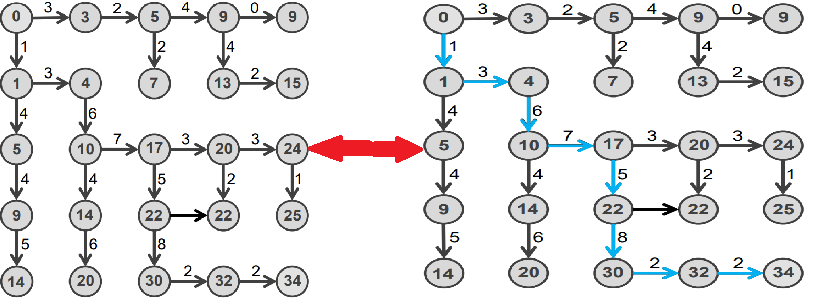
\includegraphics[width=0.7\textwidth]{poglavlja/5/slike/rek3.png}
\caption{Rekonstrukcija putanje preko putokaza kod Menhetn grafa}
\label{slika:rek3}
\end{figure}

\begin{figure}[h!]
\centering
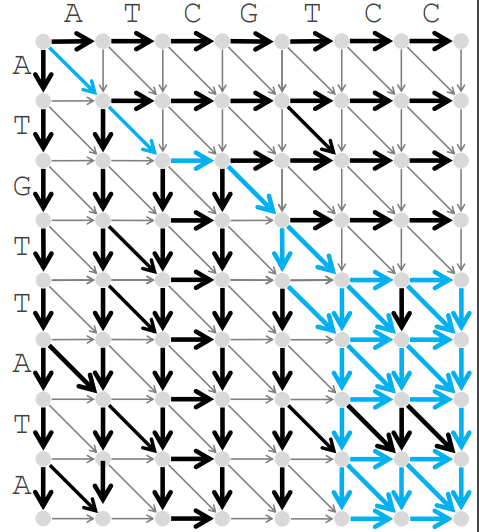
\includegraphics[width=0.5\textwidth]{poglavlja/5/slike/backtrackNajduzaZajPS.png}
\caption{Backtracking}
\label{slika:backNZPS}
\end{figure}
Sada na slici \ref{slika:backNZPS} možemo videti povratak (backtracking) kod grafa za najdužu zajedničku podsekvencu.

\subsection{Određivanje najduže zajedničke podsekvence (LCS – longest common subsequence) korišćenjem putokaza za povratak}

\begin{lstlisting}
OutputLCS (backtrack, v, i, j)
if i = 0 or j = 0
    return
if %$backtrack_i,_j$% = "%$\rightarrow$%"
    OutputLCS (backtrack, v, i, j-1)
else if %$backtrack_i,_j$% = "%$\downarrow$%"
    OutputLCS (backtrack, v, i-1, j)
else
    OutputLCS (backtrack, v, i-1, j-1)
    output  %$v_i$%
\end{lstlisting}

Do sada smo pretpostavljali da graf u kom tražimo
najdužu putanju ima samo tri vrste grana. Da li se OutputLCS može generalizovati tako da važi i za grafove koji nemaju tako specifičnu
topologiju?\\
Kako se rekurentna relacija dinamičkog programiranja menja za ovakav graf? \ref{slika:rekRel}
\begin{figure}[h]
\centering
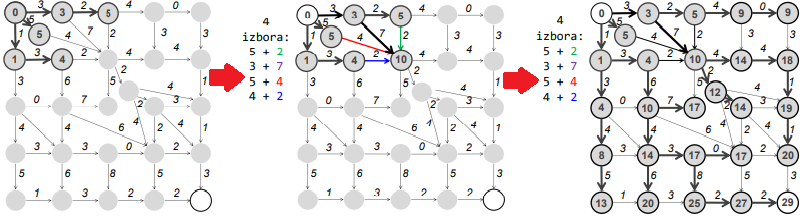
\includegraphics[width=\textwidth]{poglavlja/5/slike/rekurentaRelDinProg.png}
\caption{}
\label{slika:rekRel}
\end{figure}
\\

\textit{$s_a$ = $max_{all\ predecessors\ b\ of\ node\ a}$\{$s_b$+ weight of edge from b to a\}}
\\

Računanje skora za SVE prethodnike \ref{slika:racunanje}.

\begin{figure}[h]
\centering
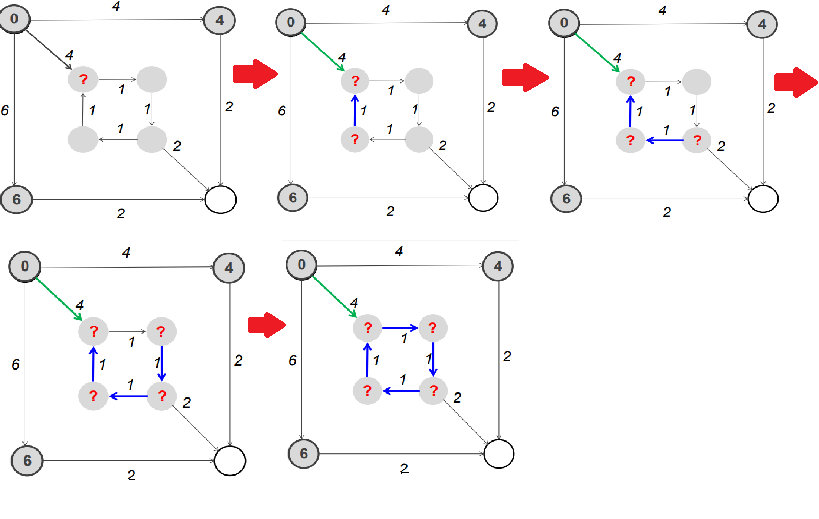
\includegraphics[width=0.7\textwidth]{poglavlja/5/slike/racunanje.png}
\caption{Začarani krug}
\label{slika:racunanje}
\end{figure}

\begin{itemize}
    \item Kod ovakve rekurentne relacije, važno je da pri računanju $s_a$ imamo izračunate $s_b$ za sve čvorove prethodnike b (čvorovi za koje
postoji grana do čvora a) Da li je to moguće u bilo kom usmerenom
težinskom grafu? Odgovor je \textbf{nije}. Da bismo kod svakog čvora mogli da mogli da izračunamo skor za sve njegove prethodnike, usmereni težinski graf mora biti acikličan. DAG (Directed Acyclic Graph) 
    \item Ako je dat usmereni aciklični graf, da li njegove čvorove možemo poređati u niz tako da njihov redosled u nizu osigurava uslov da pri računanju $s_a$ imamo izračunate $s_b$ za sve čvorove prethodnike b (čvorovi za koje postoji grana do čvora a)? Odgovor je \textbf{da}, moguće je poređati sve čvorove grafa u niz i taj niz topološki sortirati
\end{itemize}




\subsection{Topološko sortiranje}

\begin{itemize}
    \item \textbf{Topološko sortiranje} : Sortiranje čvorova DAG-a u nizu tako da sve grane u takvom nizu idu s leva na desno.
    \item \textbf{ Teorema}: Svaki DAG se može topološki sortirati.
    \item Topološko sortiranje svakog DAG-a se obavlja za O(\#edges) koraka.
\end{itemize}

\textbf{Algoritam za nalaženje najduže putanje u DAG-u>} :

\begin{lstlisting}
LongestPath(Graph, source, sink)
for each node a in Graph
     %$s_a$% %$\leftarrow$% -%$\infty$%
%$s_{source}$% %$\leftarrow$%  0
topologically order Graph
for each node a (from source to sink in topological order)
%$s_a$%  %$\leftarrow$% %$max_{all\ predecessors\ b\ of\ node\ a}$% {%$s_b$% + weight of edge from b to a}
return %$s_{sink}$%
\end{lstlisting}


\begin{itemize}
    \item Pošto svaka grana učestvuje tačno jednom, složenost je O(\#edges)
    \item LongestPath vraća dužinu najdužeg zajedničkog podniza ali ne rekonstruiše putanju
\end{itemize}

%%%%%%%%%%%%%%%%%%%%%%%jasminaaaaaa%%%%%%%%%%%%%%%%%%%%%%%%%%%%%%%%%%%%%%%%%
\section{Od globalnog do lokalnog poravnanja}

\noindent Uvedimo sledeće:
\begin{itemize}
    \item Skor poravnanja do sada - $\#\textcolor{red}{matches}$ \\
    \item Skor sa mismatch i indel kaznama - $\#\textcolor{red}{matches} - \textcolor{purple}{\mu} * \#\textcolor{purple}{mismatches} - \sigma * \#\textcolor{blue}{in}\textcolor{green}{dels}$ \\
\end{itemize}

Primer na slici \ref{slika:matriceSkora}. \\

\begin{figure}[H]
\centering
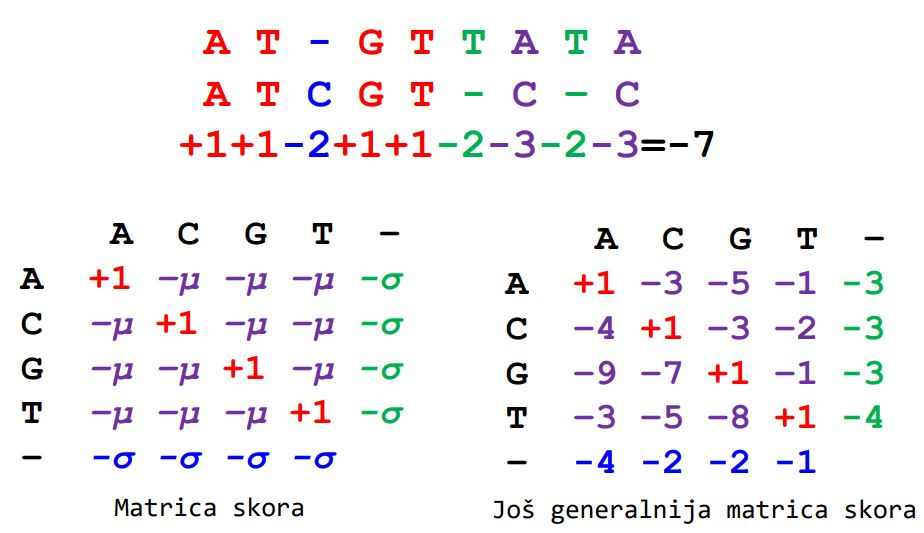
\includegraphics[width=\textwidth]{poglavlja/5/slike/matriceSkora.JPG}
\caption{}
\label{slika:matriceSkora}
\end{figure}

Navedimo rekurentnu relaciju dinamičkog programiranja kod grafa poravnanja. Počinjemo od:

$s_i,_j$ = $\max$ $\begin{cases}$
$s_{i-1},_j$ + 
$\textcolor{green}{weight\ of\ edge\ "\downarrow"\ into\ (i,j)}\\$
$s_i,_{j-1}$ + 
$\textcolor{blue}{weight\ of\ edge\ "\rightarrow"\ into\ (i,j)}\\$
$s_{i-1},_{j-1}$ + 
$\textcolor{red}{weight\ of\ edge\ "\searrow"\ into\ (i,j)}$
$\end{cases}$

Odnosno, \\
\\
$s_i,_j$ = $\max$ $\begin{cases}$
$\textcolor{green}{s_{i-1},_j - \sigma}\\$
$\textcolor{blue}{s_i,_{j-1} - \sigma}\\$
$\textcolor{red}{s_{i-1},_{j-1} + 1, v_i = w_j}\\$
$\textcolor{purple}{s_{i-1},_{j-1} - \mu, v_i \neq w_j}\\$
$\end{cases}$
\\
A uz pomoc funkcije $score()$ može se zapisati i kao: \\
\\

\begin{figure}[!htb]
     \begin{minipage}{0.49\textwidth}
        $s_i,_j$ = $\max$ $\begin{cases}$
        $\textcolor{green}{s_{i-1},_j + score(v_i, -)}\\$
        $\textcolor{blue}{s_i,_{j-1} + score(-, w_j)}\\$
        $\textcolor{red}{s_{i-1},_{j-1} score(v_i, w_j)}\\$
        $\end{cases}$
     \end{minipage}
     \hfill
     \begin{minipage}{0.49\textwidth}
       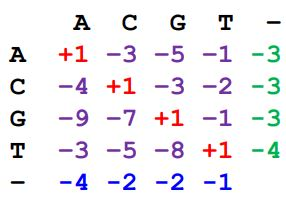
\includegraphics[width=\linewidth]{poglavlja/5/slike/rekurentna.JPG}
       \caption{}\label{}
     \end{minipage}
   \end{figure}
   
\subsection{Globalno poravnanje}

\begin{problem}[Problem globalnog poravnanja]
	Naći poravnanje sa najvišim skorom između dve niske za datu matricu skora. \\
	Ulaz: Niske v i w, kao i matrica skora score \\
	Izlaz: Poravnanje niski v i w čiji je skor poravnanja (prema matrici skora) maksimalan od svih mogućih poravnanja v i w. 
\end{problem}

\noindent Šta bi bili homeobox geni? \\
\begin{itemize}
    \item Dva gena u različitim vrstama mogu biti slična u kratkim, konzervativnim regionima, a različita u ostalim delovima.
    \item Homeobox geni sadrže kratak region homeodomen koji je čvrsto konzerviran među različitim vrstama.
    \item Globalno poravnanje može da propusti nalaženje homeodomena jer pokušava da poravna sekvence u celosti.
\end{itemize}

\noindent Uporedimo sledeća dva poravnanja: \\
\begin{figure}[!htb]
 \begin{minipage}{0.49\textwidth}
    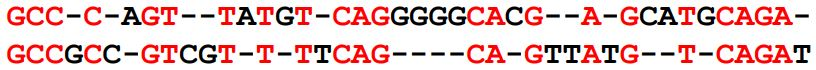
\includegraphics[width=\linewidth]{poglavlja/5/slike/globalno.JPG}
   \caption{}\label{}
   score = 22(matches) - 2(indent) = 2
 \end{minipage}
 \hfill
 \begin{minipage}{0.49\textwidth}
   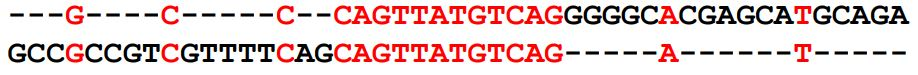
\includegraphics[width=\linewidth]{poglavlja/5/slike/lokalno.JPG}
   \caption{}\label{}
   score = 17 (matches) - 30(indent) = -13
 \end{minipage}
\end{figure}
   
\begin{figure}[!htb]
 \begin{minipage}{0.49\textwidth}
    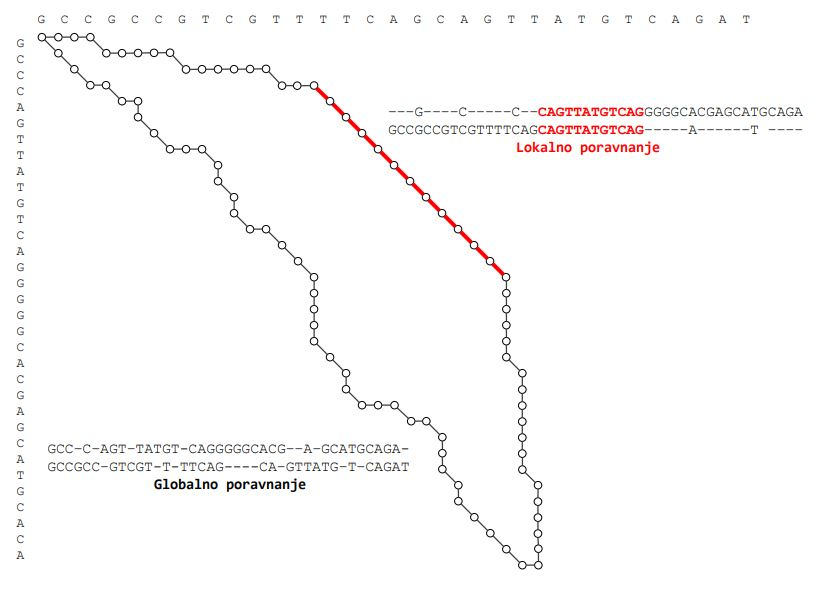
\includegraphics[width=\linewidth]{poglavlja/5/slike/grafik_poravnanje1.JPG}
   \caption{}\label{}
 \end{minipage}
 \hfill
 \begin{minipage}{0.49\textwidth}
   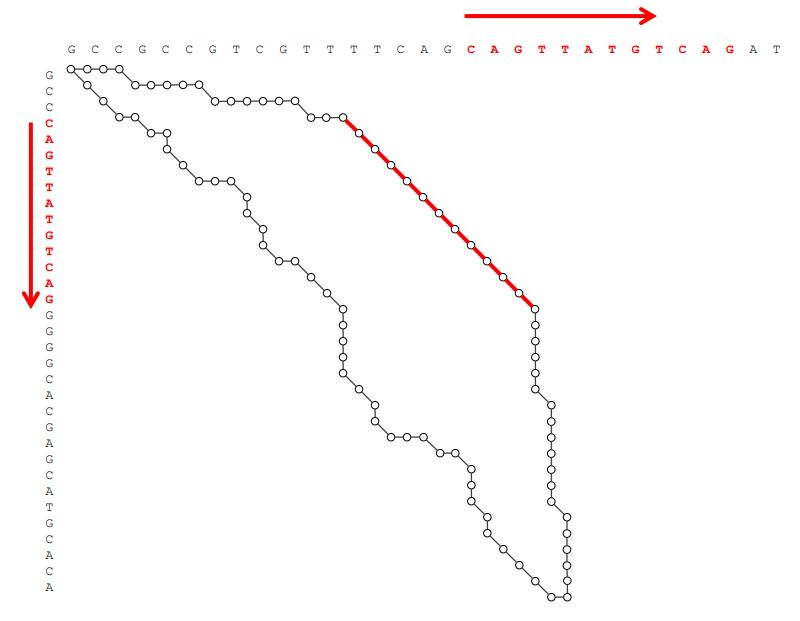
\includegraphics[width=\linewidth]{poglavlja/5/slike/grafik_poravnanje2.JPG}
   \caption{}\label{}
 \end{minipage}
\end{figure}

\noindent Ako se zapitamo koje od njih je bolje, iz priloženog zaključujemo da je to lokalno poravnanje.\\

\subsection{Lokalno poravnanje}

Lokalno poravnanje računamo kao globalno poravnanje u pravougaoniku, pogledajmo sliku \ref{slika:pravougaonici}. \\

\begin{figure}[H]
 \begin{minipage}{0.49\textwidth}
    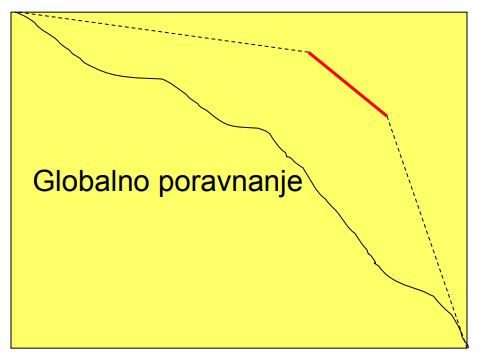
\includegraphics[width=\linewidth]{poglavlja/5/slike/lokalno_poravnanje_pravougaonici1.JPG}
   \caption{}\label{}
 \end{minipage}
 \hfill
 \begin{minipage}{0.49\textwidth}
   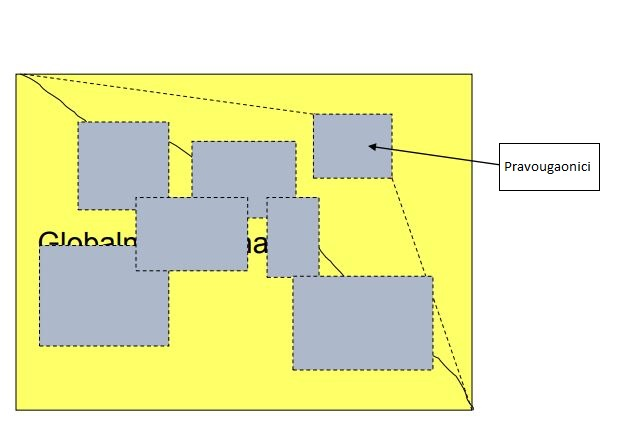
\includegraphics[width=\linewidth]{poglavlja/5/slike/lokalno_poravnanje_pravougaonici2.JPG}
   \caption{}\label{slika:pravougaonici}
 \end{minipage}
\end{figure}

\noindent Da bismo dobili lokalno poravnanje potrebno je da izračunamo globalno poravnanje u okviru svakog pravougaonika.\\
Algoritam globalnog poravnanja ponovićemo između svaka dva čvora, ne samo između početnog (source) i krajnjeg (sink). \\
Stoga, broj ponavljanja algoritma će biti $\#nodes ^ 2$ puta. \\

\begin{problem}[Problem lokalnog poravnanja]
	Naći lokalno poravnanje najvećeg skora između dve niske. \\
	Ulaz: Niske v i w, kao i matrica skora score \\
	Izlaz: Podniske niski v i w čije je globalno poravnanje (prema matrici skora) maksimalno među svim globalnim poravnanjima svih podniski niski v i w. 
\end{problem}

\noindent Zamislimo da postoji taksi koji bi nas besplatno vozio do tačke početka lokalnog poravnanja, i od tačke završetka lokalnog poravnanja pa do kraja. Na taj način ne bismo skupili negativne poene, već samo pozitivne. Ovakva vožnja nam daje samo skor lokalnog poravnanja kao što smo i želeli. \ref{slika:taksiFree}\\
 
 \begin{figure}[H]
\centering
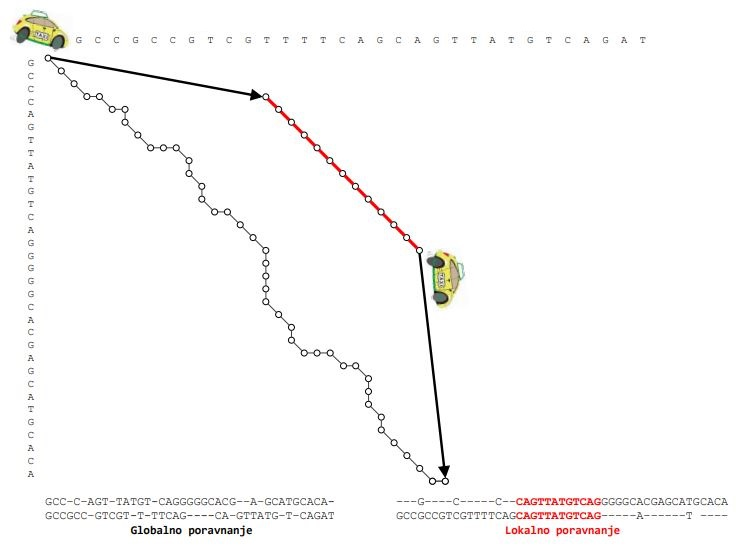
\includegraphics[width=0.7\textwidth]{poglavlja/5/slike/free_taxi.JPG}
\caption{Besplatne taksi vožnje}
\label{slika:taksiFree}
\end{figure} 

Konstruišimo Menhetn graf za problem lokalnog poravnanja: \\

\begin{figure}[H]
     \begin{minipage}{0.59\textwidth}
        Kako bi izgledao Menhetn graf za nas problem? \\
        Dodamo grane težine 0 od (0,0) do svakog čvora, i od svakog čvora do (n,m). \\
        Ukupan broj dodatih grana je $O(|v|+|w|)$, pa algoritam ostaje brz. \\
     \end{minipage}
     \hfill
     \begin{minipage}{0.39\textwidth}
       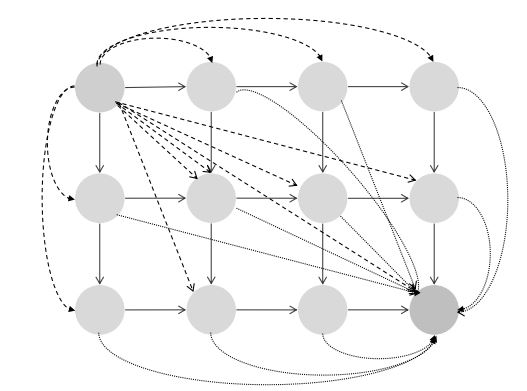
\includegraphics[width=\linewidth]{poglavlja/5/slike/free_taxi_graf.JPG}
       \caption{Menhetn graf za lokalno poravnanje}\label{}
    \end{minipage}
\end{figure}

Problem rešavamo dinamičkim programiranjem: \\

\begin{figure}[H]
     \begin{minipage}{0.59\textwidth}
        $s_i,_j$ = $\max$ $\begin{cases}$
        $s_{i-1},_j$ + 
        $\textcolor{green}{weight\ of\ edge\ "\downarrow"\ into\ (i,j)}\\$
        $s_i,_{j-1}$ + 
        $\textcolor{blue}{weight\ of\ edge\ "\rightarrow"\ into\ (i,j)}\\$
        $s_{i-1},_{j-1}$ + 
        $\textcolor{red}{weight\ of\ edge\ "\searrow"\ into\ (i,j)}$
        $\end{cases}$
     \end{minipage}
     \hfill
     \begin{minipage}{0.39\textwidth}
       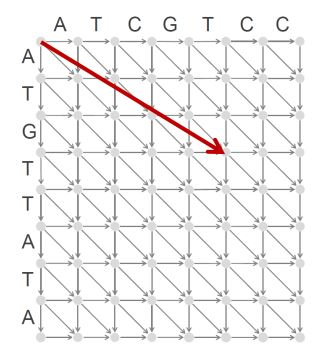
\includegraphics[width=\linewidth]{poglavlja/5/slike/lokalno_poravnanje_0.JPG}
       \caption{weight of (0,0) into (i,j) = 0}\label{}
    \end{minipage}
\end{figure}


%%%%%%%%%%%%%%%%%%%%%%%%%%%%%%%%%%%%%%%%%%%%%%%%%%%%%%%%%%%%%%%%%%%%
\section{Kažnjavanje insercija i delecija u poravnanju sekvenci}

\subsection{Kažnjavanje praznina}

\begin{itemize}
    \item U globalnom poravnanju je fiksna kazna $\sigma$ bila dodeljena svakom indelu
    \item Međutim, ova fiksna kazna može biti preoštra
kod lokalnog poravnanja kada možemo imati 100 uzastopnih indela.
    \item Niz od k uzastopnih indela često predstavlja jedan isti evolucioni događaj, ne k različitih, slika \ref{slika:kaznjavanje}
\end{itemize}

\begin{figure}[h]
\centering
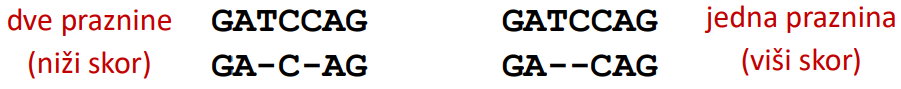
\includegraphics[width=0.5\textwidth]{poglavlja/5/slike/kaznjavanjePraznina.png}
\caption{}
\label{slika:kaznjavanje}
\end{figure}

\subsection{Adekvatnije kazne za praznine}

\textbf{Afina kazna za praznine} za prazninu dužine k:  \textbf{$\sigma+\epsilon*(k-1)$}
\begin{itemize}
    \item $\sigma$ kazna za \textbf{otvaranje} praznine
    \item $\epsilon$ kazna za \textbf{proširenje} praznine
    \item $ \sigma > \epsilon$ , jer otvaranje praznine treba kazniti više nego njeno proširenje
\end{itemize}



U slici \ref{slika:modelovanje} prikayano je modelovanje afinih kazni za praznine pomoću dugih grana.

\begin{figure}[h!]
\centering
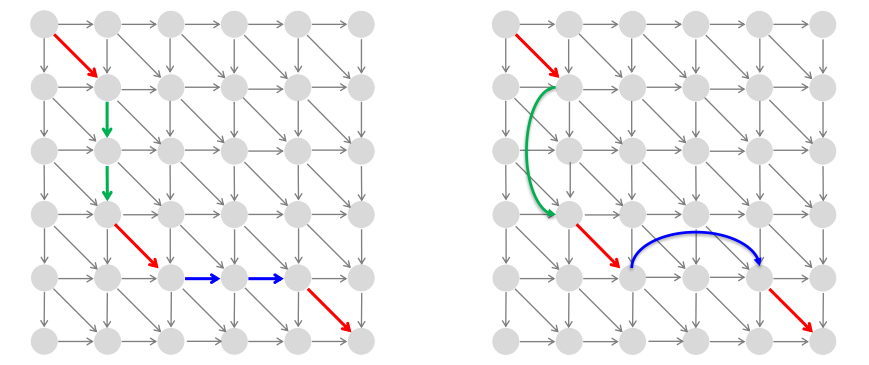
\includegraphics[width=0.7\textwidth]{poglavlja/5/slike/modelovanjePomocuDugihGrana.png}
\caption{Modelovanje afinih kazni za praznine pomoću dugih grana}
\label{slika:modelovanje}
\end{figure}

\subsection{Izgradnja Menhetn grafa sa afinim kaznama za praznine}

\begin{figure}[h!]
\centering
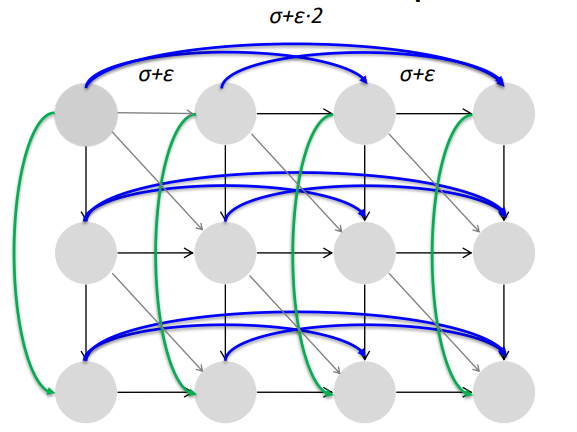
\includegraphics[width=0.5\textwidth]{poglavlja/5/slike/MenhettnAifnePraznine.png}
\caption{Dodali smo $O(n^3)$ grana}
\label{slika:afiniMenhetn}
\end{figure}


\begin{itemize}
    \item Vremenska složenost je direktno proporcionalna broju grana, zbog čega želimo da smanjimo broj grana u grafu (trenutno je
$O(n^3)$ \ref{slika:afiniMenhetn})
\item Jedan način za smanjivanje broja grana je povećanje broja čvorova u grafu
\item Zato delimo Menhetn graf na tri nivoa \ref{slika:triNivoa}
\end{itemize}


\begin{figure}[h!]
\centering
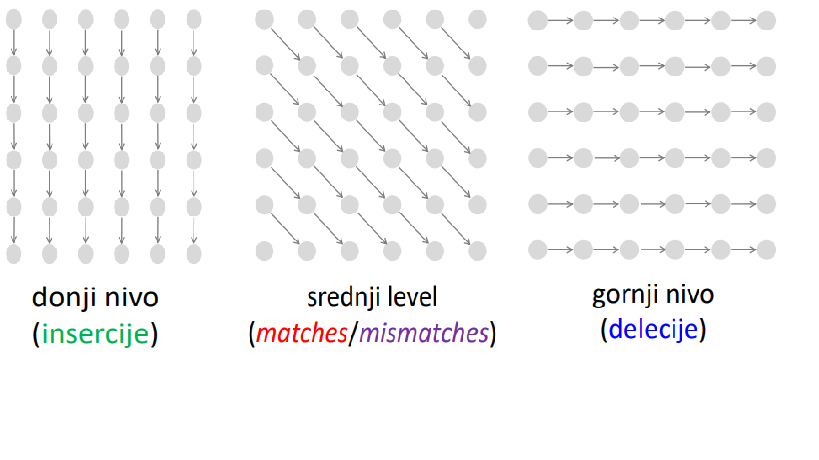
\includegraphics[width=\textwidth]{poglavlja/5/slike/triNivoa.png}
\caption{Podela Menhetna grafa na 3 nivoa}
\label{slika:triNivoa}
\end{figure}

Ako imamo putanju poput one na slici \ref{slika:kakoSimulirati}, kako da je predstavimo pomoću Menhetn grafa na 3 nivoa? Rešenje je prikazano na slici \ref{slika:simulacija}


\begin{figure}[h!]
\centering
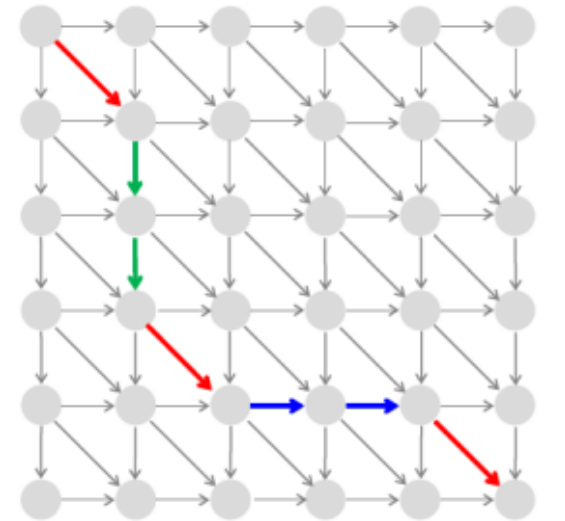
\includegraphics[width=0.5\textwidth]{poglavlja/5/slike/kakoSimulirari.png}
\caption{Kako predstaviti pomoću Menhetn grafa na 3 nivoa?}
\label{slika:kakoSimulirati}
\end{figure}


\begin{figure}[h!]
\centering
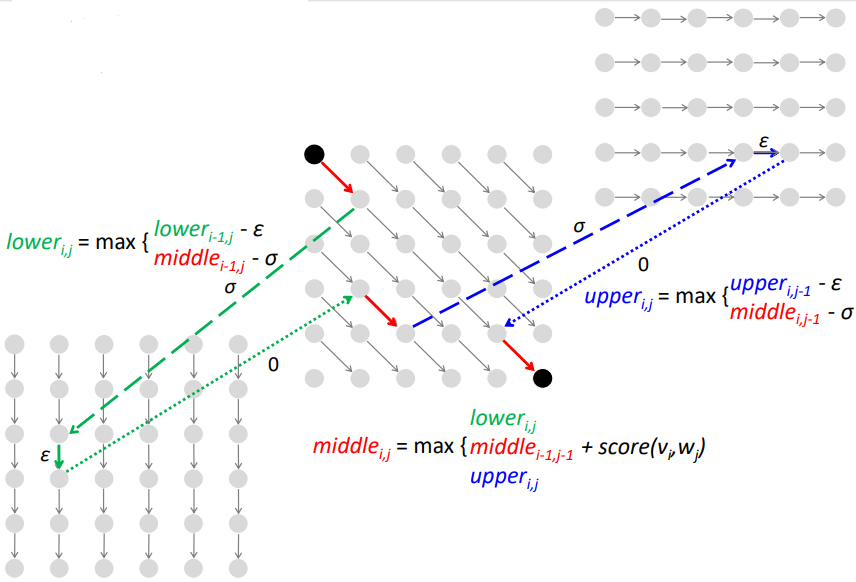
\includegraphics[width=0.7\textwidth]{poglavlja/5/slike/simulacija.png}
\caption{Simulacija Menhetn grafa na 3 nivoa}
\label{slika:simulacija}
\end{figure}

%%%%%%%%%%%%%%%%%%%%%%%%%%%%%%%%%jasminaaaa%%%%%%%%%%%%%%%%%%%%%%%%%%%%%%%%%%%

\section{Prostorno efikasno poravnanje sekvenci}

Zapitajmo se sledeće: \\
Da li možemo poravnati NPR sintetaze iz dve različite bakterije? \\
\\

Uzmimo u obzir sledeće činjenice:
\begin{itemize}
    \item NPR sintetaze su obično veoma dugi proteini, približno 20 000 aminokiselina
    \item Vremenska složenost poravnanja je probližno jednaka broju ivica (\#edges), odnosno kvadratna
    \item Prostorna složenost poravnanja je probližno jednaka broju čvorova (\#nodes), odnosno kvadratna
    \item \textbf{Memorija je često usko grlo pri poređenju dugih sekvenci}
\end{itemize}

Iz prethodnog zaključujemo da nam prostorna složensot pravi problem i da bi za prosečan racunar ovo bilo nemoguće da izračuna. 
Stoga, potreban nam je drugi pristup koji će nam rešiti problem. Potreban nam je algoritam koji zahteva linearnu prostornu složenost i udvostručenu vremensku složenost. U te svrhe najčešće se koristi algoritam koji radi po principu podeli-pa-vladaj. \\

Uvedimo nove pojmove:
\begin{itemize}
    \item Srednja kolona poravnanja (middle) $= \#columns/2$, slika \ref{slika:srednjaKolona}
    \item Srednji čvor poravnanja - čvor u preseku putanje optimalnog poravnanja i srednje kolone, slika \ref{slika:srednjiCvor}
\end{itemize}


\begin{figure}[h!]
\centering
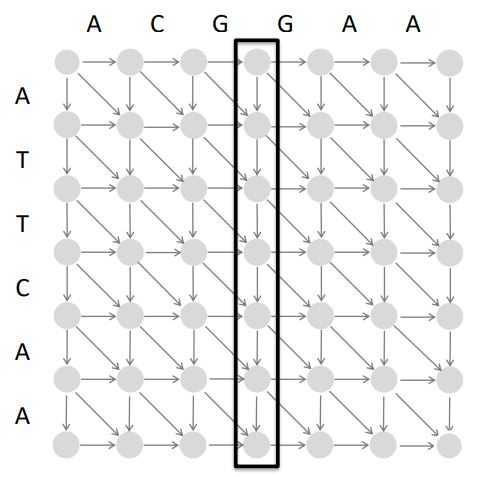
\includegraphics[width=0.5\textwidth]{poglavlja/5/slike/srednjaKolona.JPG}
\caption{Srednja kolona poravnanja}
\label{slika:srednjaKolona}
\end{figure}

\begin{figure}[h!]
\centering
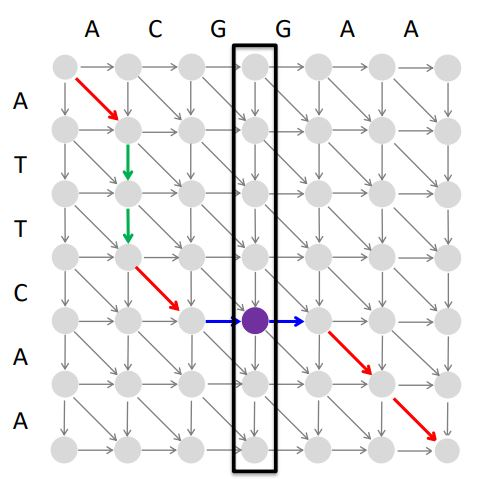
\includegraphics[width=0.5\textwidth]{poglavlja/5/slike/srednjiCvor.JPG}
\caption{Srednji čvor poravnanja}
\label{slika:srednjiCvor}
\end{figure}

Koristeći navedene pojmove, demonstrirajmo algoritam \textbf{Podeli-pa-vladaj} za poravnanje sekvenci, slika \ref{slika:podeliPaVladaj}: \\

\begin{lstlisting}
AlignmentPath(source, sink)
    find middleNode
    AlignmentPath(source, middleNode)
    AlignmentPath(middle, sink)
\end{lstlisting}

\begin{figure}[h!]
\centering
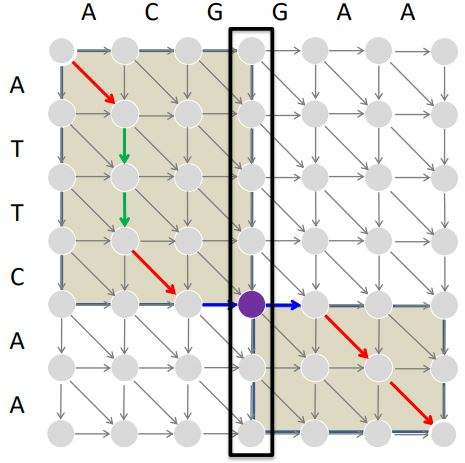
\includegraphics[width=0.5\textwidth]{poglavlja/5/slike/podeliPaVladaj.JPG}
\caption{Srednja kolona poravnanja}
\label{slika:podeliPaVladaj}
\end{figure}

\subsection{Prostorna složenost}
Za nalaženje najduže putanje u grafu poravnanja traži se čuvanje svih putokaza za - $O(nm)$ prostora. \\
Međutim, za nalaženje dužine najduže putanje u grafu poravnanja ne traži se čuvanje svih putokaza - $O(n)$ prostora, slika \ref{slika:prostornaSlozenost}

\begin{figure}[h!]
\centering
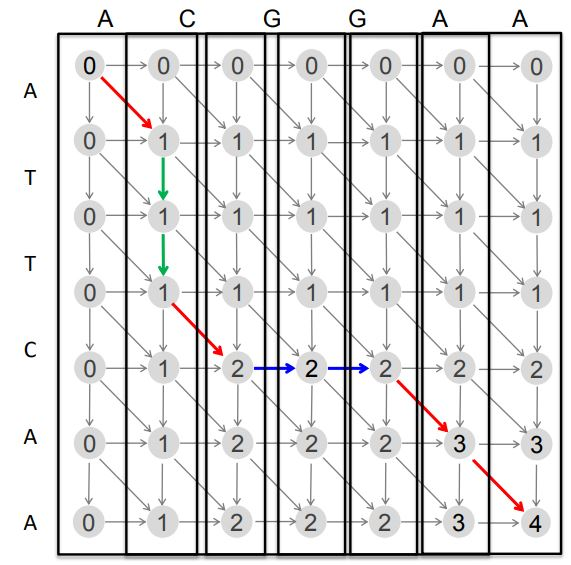
\includegraphics[width=0.5\textwidth]{poglavlja/5/slike/prostornaSlozenost2.JPG}
\caption{Recikliranje prostora za kolone u grafu poravnanja}
\label{slika:prostornaSlozenost}
\end{figure}

Dobijamo da je prostor potreban za algoritam $2*n \sim O(n)$, odnosno, linearan. \\ 

\subsection{Vremenska složenost}

Neka je \textbf{i-putanja} najduža putanja od svih putanja koja posećuje i-ti čvor u srednjoj koloni i neka je \textbf{$length(i)$} dužina i-putanje.\\

Na slici \ref{slika:iputanja} vidimo da je $length(0)=2$ i $length(4)=4$. \\


\begin{figure}[h!]
\centering
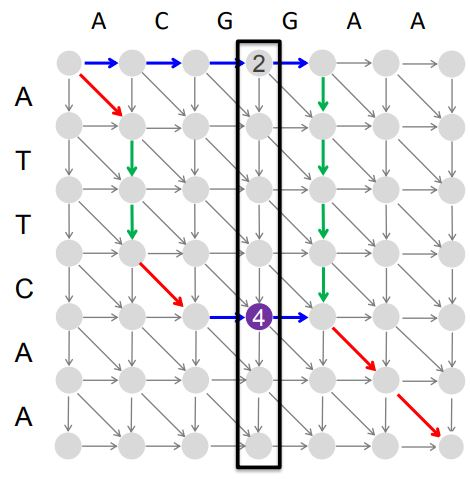
\includegraphics[width=0.5\textwidth]{poglavlja/5/slike/i_putanje.JPG}
\caption{Računanje length(i)}
\label{slika:iputanja}
\end{figure}


$length(i)$ možemo računati na sledeći način:
\begin{center}
$length(i) = fromSource(i) + toSink(i)$
\end{center}

\begin{figure}[h!]
\centering
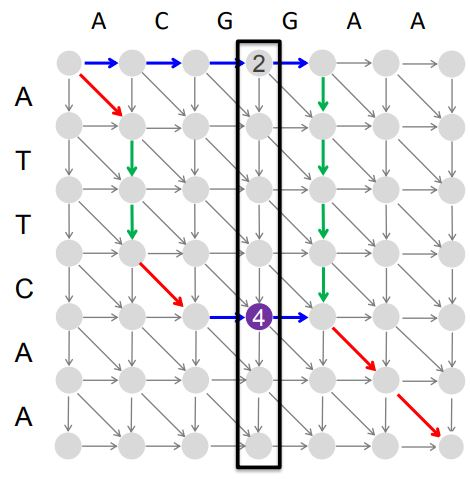
\includegraphics[width=0.5\textwidth]{poglavlja/5/slike/i_putanje.JPG}
\caption{Računanje length(i)}
\label{slika:iputanja}
\end{figure}

Na slici \ref{slika:sourceSink} vidimo koliko je potrebno vremena za nalaženje srednjeg čvora - čak $O(nm)$ vremena za nalaženje samo jednog čvora! 
\begin{figure}[h!]
\centering
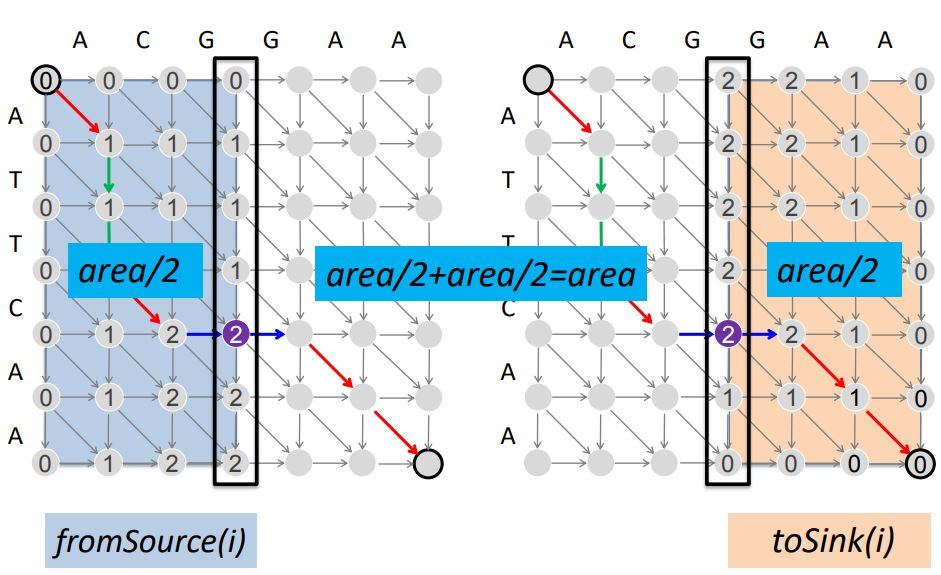
\includegraphics[width=0.5\textwidth]{poglavlja/5/slike/sourceSink.JPG}
\caption{Računanje vremena za nalaženje srednjeg čvora}
\label{slika:sourceSink}
\end{figure}

Svaki problem se može rešiti u vremenu proporcionalnom broju grana tj. površini koju zauzima. \\
Vreme potrebno za rešavanje naredna dva potproblema: $area/4 + area/4 = area/2$, znači  $O(nm + nm/2)$ vremena za nalaženje 3 čvora. \\
Dakle, vreme potrebno za nalaženje svih čvorova je: $area + area/2 + area/4 + area/8 + \dots < 2 * area$! Slika \ref{slika:vreme} vizuelno prikazuje vreme potrebno za nalaženje 7 tačaka. \\

\begin{figure}[h!]
\centering
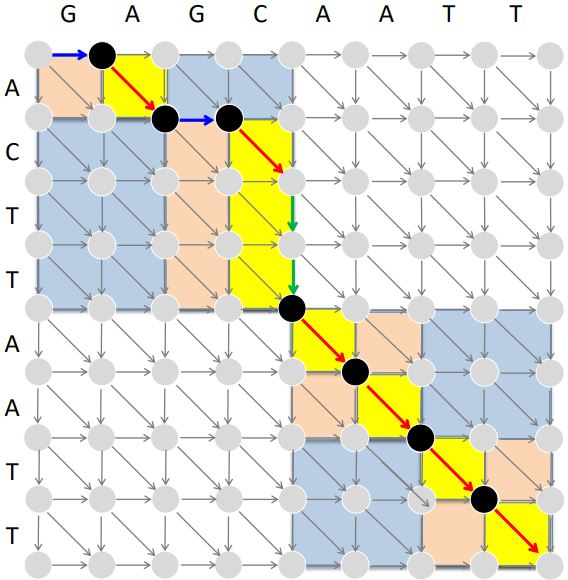
\includegraphics[width=0.5\textwidth]{poglavlja/5/slike/vremenskaSlozenostPPV.JPG}
\caption{Računanje vremena za nalaženje 7 tačaka}
\label{slika:vreme}
\end{figure}

Pokazali smo da je vremenska složenost $2*n*m \sim O(n*m)$. \\
%%%%%%%%%%%%%%%%%%%%%%%%%%%%%%%%%%%%%%%%%%%%%%%%%%%%%%%%%%%%%%%%%%%%

\section{Višestruko poravnanje sekvenci}

\subsection{Od dvostrukog do višestrukog poravnanja}
\begin{itemize}
    \item Do sada su u poravnanju učestvovale samo dve sekvence.
    \item Slaba sličnost između dve sekvence postaje značajna ako je prisutna i u drugim sekvencama
    \item Višestruka poravnanja mogu otkriti suptilne sličnosti koje dvostruka poravnanja ignorišu
\end{itemize}

\subsection{Poravnanje tri A-domena}
Na slici \ref{slika:poravnavanjaTriA} je prikazano poravnanje tri A-domena
\begin{figure}[h!]
\centering
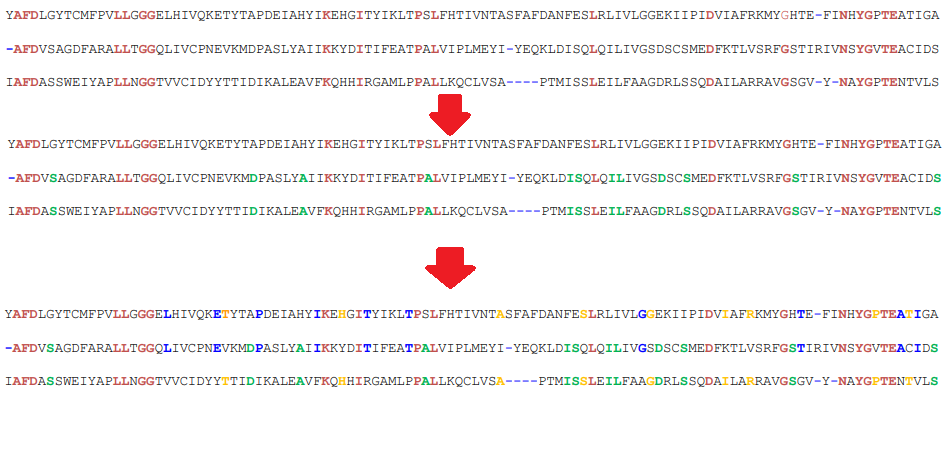
\includegraphics[width=\textwidth]{poglavlja/5/slike/poravnavanjaTriAdomena.png}
\caption{Poravnavanja 3 A-domena}
\label{slika:poravnavanjaTriA}
\end{figure}

\subsection{Generalizacija dvostrukog na višestroko poravnanje}
    
\begin{itemize}
    \item Poravnanje 2 sekvence je matrica od 2 reda
    \item Poravnanje 3 sekvence je matrica od 3 reda (slika  \ref{slika:poravnavanjeMatrica})
    \begin{figure}[h!]
    \centering
    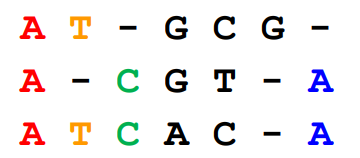
\includegraphics[width=0.3\textwidth]{poglavlja/5/slike/poravnanjeMatrica.png}
    \caption{}
    \label{slika:poravnavanjeMatrica}
    \end{figure}
    \item Funkcija skora treba da dodeljuje visok skor poravnanjima sa konzerviranim kolonama
\end{itemize}



\subsection{Poravnanja = 3-D putanje}

Poravnanje sekvenci ATGC, AATC i ATGC \ref{slika:3d}

\begin{figure}[h]
\centering
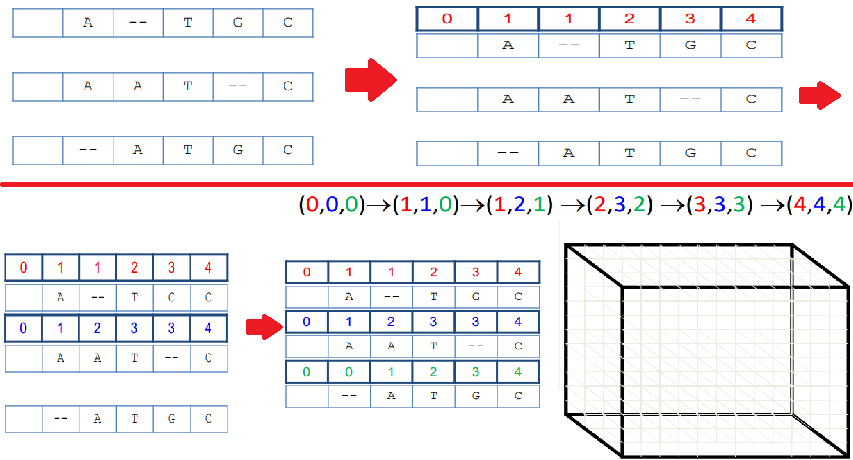
\includegraphics[width=0.8\textwidth]{poglavlja/5/slike/3dPoravnanja.png}
\caption{Poravnanje sekvenci ATGC, AATC i ATGC}
\label{slika:3d}
\end{figure}

\subsection{2-D poravnanje u odnosu na 3-D poravnanje}
\begin{figure}[h]
\centering
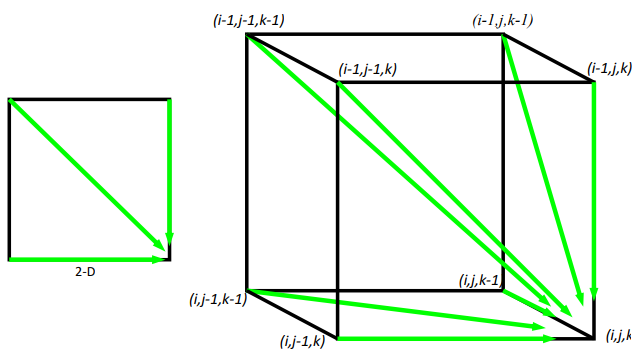
\includegraphics[width=0.5\textwidth]{poglavlja/5/slike/2d3d.png}
\caption{}
\label{slika:2d3d}
\end{figure}
2-D poravnanje u odnosu na 3-D poravnanje prikazano na slici \ref{slika:2d3d}.

\subsection{Rekurentna relacija dinamičkog programiranja
za višestruko poravnanje}



$s_i,_j,_k$ = $\max$ $\begin{cases}$

$s_{i-1},_{j-1},_{k-1}$+ $\delta(v_i, w_j, u_k)\\$
$s_{i-1},_{j-1},_k$+ $\delta(v_i, w_j, -)\\$
$s_{i-1},_j,_{k-1}$+ $\delta(v_i, -, u_k)\\$
$s_i,_{j-1},_{k-1}$+ $\delta(-, w_j, u_k)\\$
$s_{i-1},_{j},_k$+ $\delta(v_i,-, -)\\$
$s_{i},_{j-1},_k$+ $\delta(-, w_j, -)\\$
$s_{i},_{j},_{k-1}$+ $\delta(-, -, u_k)\\$
$\end{cases}$

$\delta$(x, y, z) - element 3-D matrice skora

\subsection{Vremenska složenost dinamičkog algoritma
za višestruko poravnanje}

\begin{itemize}
    \item Kao kod dvostrukog poravnanja, vremenska složenost je proporcionalna broju grana O(\#edges)
    \item Za 3 sekvence n, vremenska složenost je proporcionalna 7$n^3$
    \item Za poravnanje k sekvenci, potrebno je izgraditi kdimenzionalni Menhetn graf sa: 
    \begin{itemize}
        \item  $n^k$ čvorova
        \item većina čvorova će imati $2^k – 1$ ulaznih grana
        \item Vremenska složenost: O($2^kn^k$)
    \end{itemize}
\end{itemize}


Višestruko poravnanje uključuje i dvostruko poravnanje, slika \ref{slika:visestrukoDvostruko}

\begin{figure}[h!]
\centering
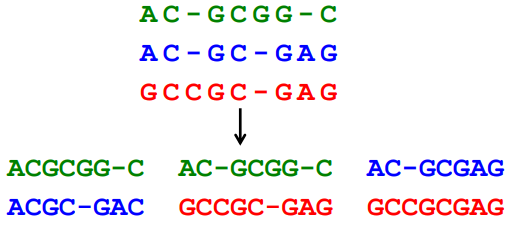
\includegraphics[width=0.5\textwidth]{poglavlja/5/slike/visestrukoDvostruko.png}
\caption{}
\label{slika:visestrukoDvostruko}
\end{figure}

\subsection{Da li se višestruko poravnanje može izgraditi iz dvostrukog?}
Za dati skup proizvoljnih dvostrukih poravnanja, možemo li konstruisati višestruko poravnanje iz kog su izvedeni (slika \ref{slika:dvostruka})?

\begin{figure}[h!]
\centering

\includegraphics[width=0.7\textwidth]{poglavlja/5/slike/dvostruka.png}
\caption{}
\label{slika:dvostruka}
\end{figure}

\subsection{Profilna reprezentacija višestrukog poravnanja}

Na slici \ref{slika:profilVisetruko} prikazana profilna reprezentacija višestrukog poravnanja.
\begin{figure}[h!]
\centering
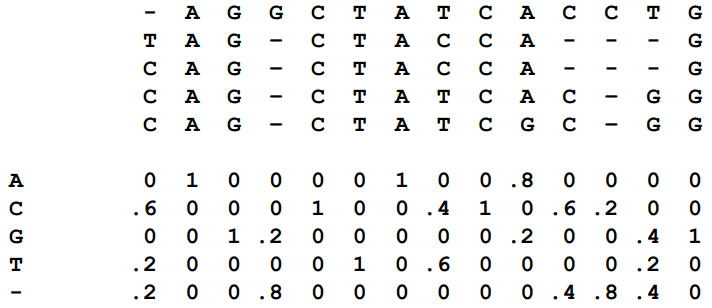
\includegraphics[width=0.6\textwidth]{poglavlja/5/slike/profilVisestruko.png}
\caption{}
\label{slika:profilVisetruko}
\end{figure}


\begin{itemize}
    \item Do sada smo poravnavali \textbf{sekvencu u odnosu na sekvencu.}
    \begin{itemize}
        \item Možemo li poravnati \textbf{sekvencu u odnosu na profil}?
        \item Možemo li poravnati \textbf{profil u odnosu na profil}?
    \end{itemize}
   
\end{itemize}


\subsection{Višestruko poravnanje: pohlepni pristup}

\begin{itemize}
    \item Izabrati najsličnije sekvence i kombinovati ih u profil
     \item Tako bismo smanjili broj sekvenci sa k na k-2 i jedan profil
    \item Iterirati
\end{itemize}

Primer pohlepnog pristupa:
\begin{itemize}
    \item Sekvence: GATTCA, GTCTGA, GATATT, GTCAGC
    \item 6 dvostrukih poravnanja (\textcolor{red}{match}+1, \textcolor{ForestGreen}{in}\textcolor{blue}{dels} i \textcolor{purple}{mismatches -1}) slika \ref{slika:sestDvostrukih}
    \begin{figure}[h!]
    \centering
    \includegraphics[width=0.5\textwidth]{poglavlja/5/slike/sestDvostrukih.png}
    \caption{}
    \label{slika:sestDvostrukih}
    \end{figure}
    \item Pošto su $s_2$ i $s_4$ najbliže, od njih pravimo profil
    
     \begin{figure}[h!]
    \centering
    \includegraphics[width=0.4\textwidth]{poglavlja/5/slike/profil.png}
    \caption{}
    \label{slika:profil}
    \end{figure}
    \item Novi skup od 3 sekvence za poravnanje:\\
            $s_1$ GATTCA\\
            $s_3$ GATATT\\
            $s_2,_4$ \textcolor{ForestGreen}{GTC}\textcolor{red}{t/a}\textcolor{ForestGreen}{G}\textcolor{red}{a/c}

\end{itemize}
%%% dodati tekst


%%%%%%%%%%%%%%%%%%%%%%%%%%%%%%%%%%%%%%%%%%%%%%%%%%%%%%%%%%%%%%%%%%%

\newpage
\section{Zadaci sa vežbi}
\setexamplecodestyle

U nastavku će biti predstavljeni zadaci sa vežbi na kursu rađeni u programskom jeziku Python.

\subsection{Manhattan Tourist}

\lstinputlisting[language=Python]{poglavlja/5/kodovi/ManhattanTourist.py}

\subsection{LCS Backtrack}

\lstinputlisting[language=Python]{poglavlja/5/kodovi/LCSBacktrack.py}

\subsection{Global Alignment}

\lstinputlisting[language=Python]{poglavlja/5/kodovi/GlobalAlignment.py}

\subsection{Local Alignment}

\lstinputlisting[language=Python]{poglavlja/5/kodovi/LocalAlignment.py}

\subsection{Edit Distance}

\lstinputlisting[language=Python]{poglavlja/5/kodovi/EditDistance.py}